\documentclass[a4paper,14pt]{extarticle} \usepackage[utf8]{inputenc}
\usepackage[T1]{fontenc}
\usepackage[margin=2.5cm]{geometry}

% Fonte Caladea se existir, senão lmodern
\IfFileExists{caladea.sty}{
  \usepackage{caladea}
}{
  \usepackage{lmodern} }
\usepackage{ragged2e}
\usepackage{graphicx}
\usepackage[portuguese]{babel}
\usepackage{wrapfig}
\usepackage{hyperref}
\usepackage{fancyhdr}
\usepackage{xcolor}
\usepackage{rotating}
\usepackage{titlesec}
\usepackage{epigraph}
\usepackage{dirtytalk}
\usepackage{indentfirst} % Indenta o primeiro parágrafo após seções

% Ajuste do recuo de parágrafo
\setlength{\parindent}{1.5em}

% Adjust headheight to remove LaTeX warning
\setlength{\headheight}{17.54163pt}

% Centralizar títulos
\titleformat{\section}
  {\normalfont\centering\bfseries\Large}{}{1em}{}

\titleformat{\subsection}
  {\normalfont\centering\bfseries\large}{}{1em}{}

\titleformat{\subsubsection}
  {\normalfont\centering\bfseries}{}{1em}{}

% -------------- Símbolos de Versículo e Resposta --------------
% Definição do símbolo (a “barrinha” inclinada)
\makeatletter
\newcommand{\vers@resp@sym}{%
  \raisebox{0.2ex}{\rotatebox[origin=c]{-20}{$\m@th\rceil$}}%
}
% macro interna que sobrepõe a barrinha e a letra V ou R
\newcommand{\vers@resp}[2]{%
  {\ooalign{%
     \hidewidth\kern#1\vers@resp@sym\hidewidth\cr
     #2\cr
  }}%
}
% comandos públicos \versicle e \response
\DeclareRobustCommand{\versicle}{\vers@resp{-0.1em}{V}}
\DeclareRobustCommand{\response}{\vers@resp{0pt}{R}}
\makeatother
% ^------------- Símbolos de Versículo e Resposta -------------^

% Rodapé com imagem e página
\pagestyle{fancy}
% ---- Cabeçalho ------------
\fancyhf[C]{}
% ----- Rodapé --------------
\fancyfoot[C]{%
  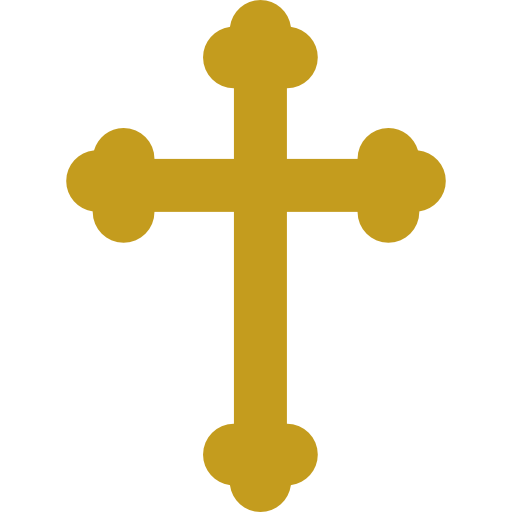
\includegraphics[scale=0.2]{assets/cross.png}\quad
  \textit{\textit{São Cirilo e São Metódio, Rogai por Nós}}\quad
  \thepage
}

\usepackage{pdfpages}
\begin{document}
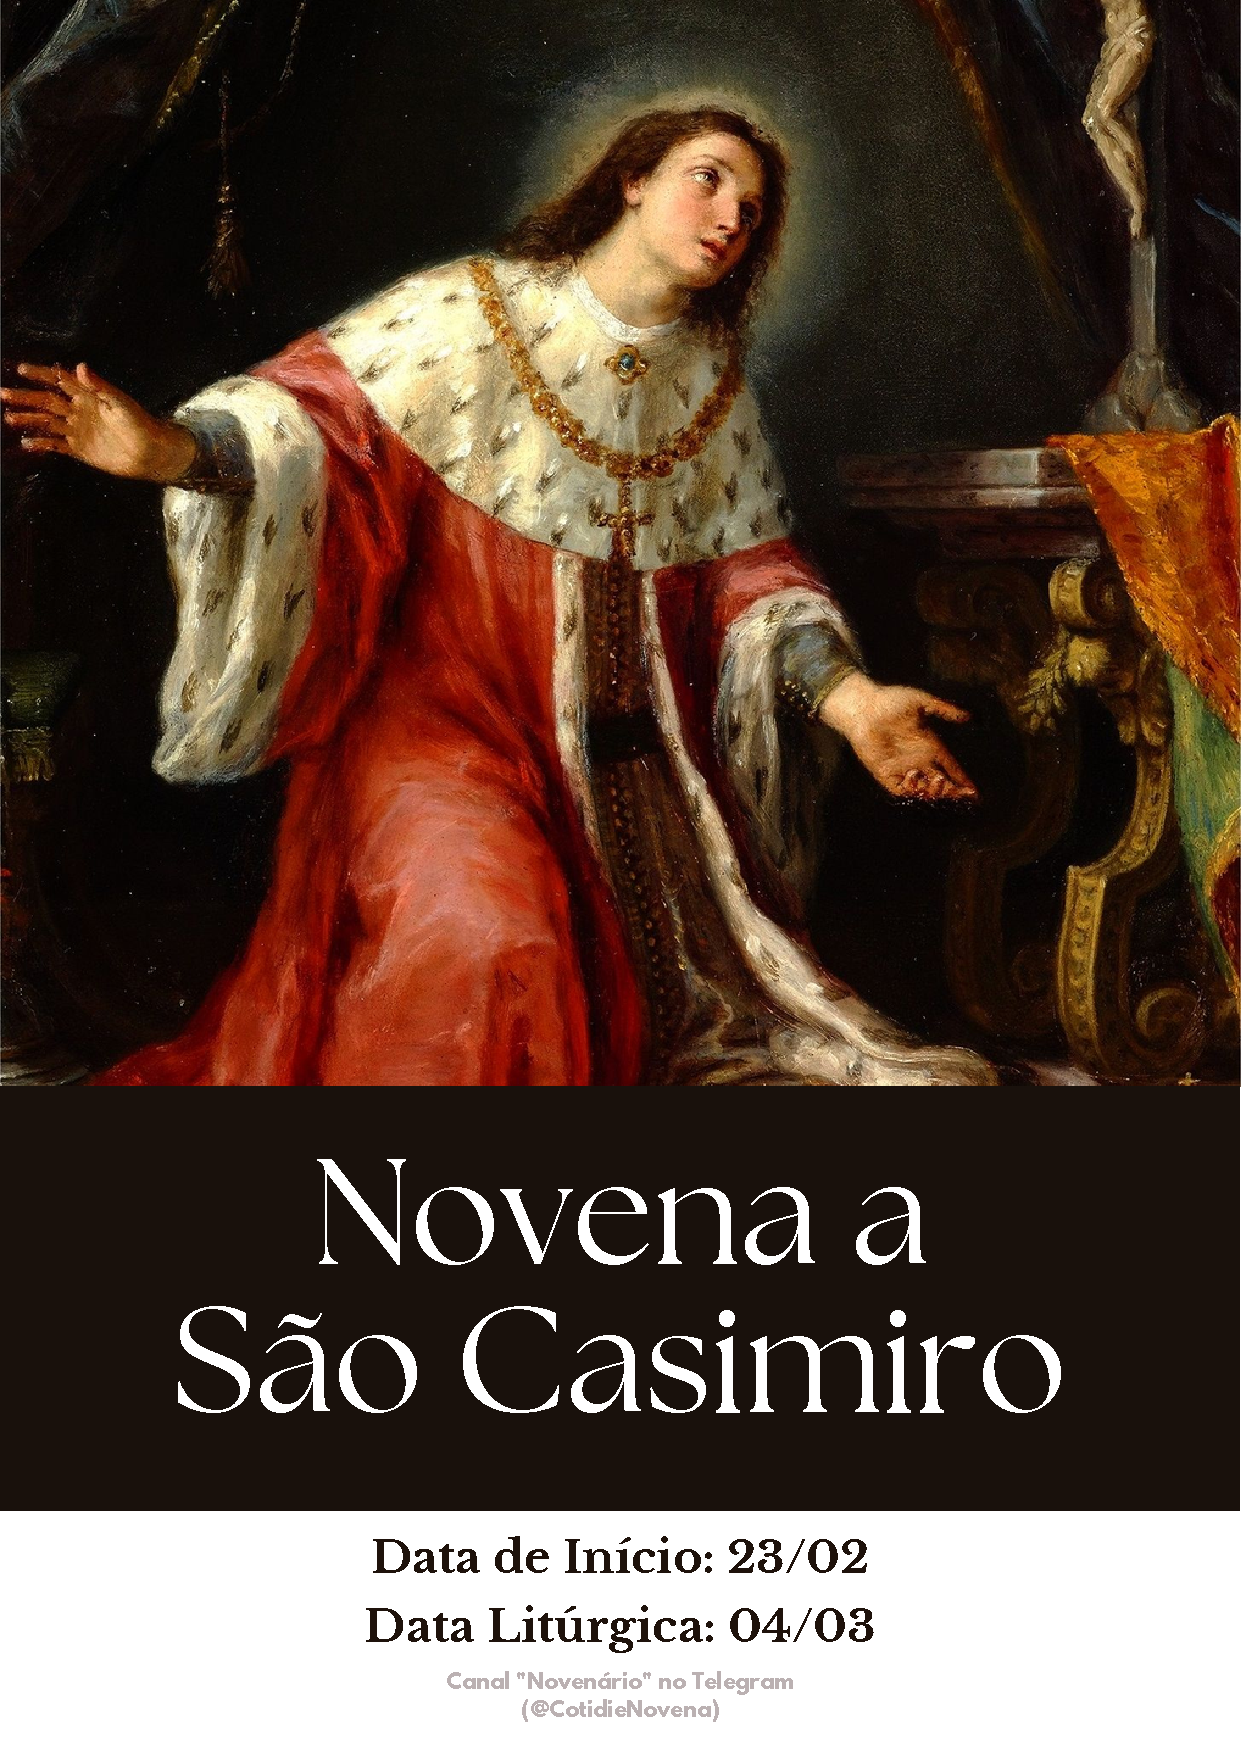
\includepdf[pages=1]{Capa São Casimiro}

\begin{center}
  {\huge Novena de São Casimiro}
\end{center}



\noindent\rule{\textwidth}{0.4pt}

\tableofcontents

\thispagestyle{empty}


% --- Origem ---
\newpage

\section{História}

\subsection{Origens}

Casimiro nasceu no dia 03 de outubro de 1458, na Croácia. Foi o décimo terceiro filho do rei Casimiro IV, da Polônia. Sua mãe era a rainha Elisabete d'Asburgo. Ele tinha o direito de assumir um território na Polônia e reinar sobre ele, mas preferiu seguir o caminho do amor e da caridade.
App Cruz Terra Santa

\subsection{Chamado desde pequeno}

Desde pequeno Casimiro procurou a simplicidade e abriu mão do luxo da realeza. As ricas festas e as facilidades da nobreza não o seduziam. Ainda adolescente, optou por fazer um voto de castidade e por viver uma vida simples recolhido no seu quarto. Seu quarto, aliás, foi transformado numa cela, como seria a de um eremita. Ali, Casimiro dedicou-se à oração, à penitência, a disciplina e à solidão. Esta sua vocação foi notada desde a infância.

\subsection{Recusa uma coroa}

Quando Casimiro tinha apenas treze anos, os húngaros depuseram o rei Mateus Corvino e ofereceram a coroa a Casimiro. Ele, porém, recusou por não buscar o poder e também porque seu pai não era a favor daquela deposição. A única “ambição” de Casimiro era, de fato, o ideal monástico, a vida de oração e a santidade.

\subsection{Cumprindo deveres políticos}

O jovem Casimiro, no entanto, não se eximia de deveres políticos que estivessem ao seu alcance e que não o desviassem de sua vocação. Assim, ajudado seu pai nos assuntos do reino a partir dos dezessete anos. Ajudou a resolver problemas da Lituânia e se tornou muito querido por todos de lá. Mas ele não queria nenhuma coroa. Quando o rei da Hungria se converteu ao cristianismo e deixou tudo para ingressar num mosteiro, o pai de Casimiro, o rei Casimiro IV, passou a ser o dono daquelas terras, que incluíam a então Prússia e a Hungria. Nem assim o jovem Casimiro quis reinar sobre esses territórios.

\subsection{Governante por um tempo}

O pai de Casimiro teve que se ausentar da sede do reino para negociar a ampliação do reino até aos mares Negro e Báltico, tornando seu império gigantesco. Por isso, confiou a regência da sede ao filho Casimiro. O filho, cumpriu suas obrigações com grande competência e passou a ser mais amado pelo povo. Porém, o poder não o seduziu. Assim, quando seu pai voltou, entregou o poder com alívio, preferindo a caridade para com os pobres e a vida simples.

\subsection{Rejeitando um casamento}

O pai de São Casimiro negociou um casamento para o filho. Seria com uma bela princesa de um reino vizinho e amigo. São Casimiro, porém, recusou, alegando que sua vocação era para a vida celibatária e uma dedicação total a Deus e aos pobres. A contragosto, seu pai desfez o contrato de casamento e Casimiro seguiu sua vocação.

\subsection{Morte}

São Casimiro faleceu com apenas vinte e cinco anos, vítima de tuberculose. Seu corpo foi sepultado na cidade de Vilnius, capital da Lituânia. Era o dia 04 de março de 1484. Em pouco tempo ele começou a ser venerado pelos povos da Polônia, Lituânia, Hungria e Rússia. O culto a São Casimiro foi introduzido na Europa ocidental por peregrinos que iam visitar sua sepultura e se encantavam com sua história. Sua canonização foi celebrada pelo Papa Leão X. Depois disso, passou a ser o padroeiro da Lituânia e da Polônia. Ele também é o Padroeiro da juventude Lituana e protetor dos pobres.

% --- Orações Diárias ---
\newpage

\vfill

\section{Orações}
\subsection{Oração Inicial}\label{sub:inicial} % (fold)

Ó Deus, que destes a São Casimiro o dom da santidade e o zelo pela salvação das almas, concedei-nos, por sua intercessão, a graça de viver segundo o Vosso Santo Evangelho. Que ele, que foi um exemplo de pureza, devoção e amor aos pobres, nos inspire a buscar a santidade em nossa vida.

Neste momento, apresento a Vós, Senhor, as minhas intenções particulares:
\textit{(faça aqui o seu pedido ou coloque suas intenções).}

\subsection{Dia 1 - A Pureza de Coração}

\underline{\nameref{sub:inicial}}

São Casimiro é um modelo de pureza e castidade. Ele guardou seu coração puro, dedicando-se inteiramente a Deus e à Virgem Maria. Sua vida nos ensina que a pureza é um caminho de santidade e felicidade.
Ó São Casimiro, que guardastes a pureza de coração como um tesouro precioso, ajuda-me a viver uma vida casta e pura, longe das tentações do mundo. Ensina-me a amar a Deus com todo o meu ser e a buscar a santidade em minha juventude. Amém.


\underline{\nameref{sub:final}}

\subsection{Dia 2 - A Devoção à Eucaristia}

\underline{\nameref{sub:inicial}}

São Casimiro tinha uma profunda devoção à Eucaristia, encontrando nela a força para sua vida espiritual. Ele nos ensina que Jesus Eucarístico é o alimento da alma e a fonte de toda graça.
Ó São Casimiro, que amastes a Eucaristia com todo o teu coração, ajuda-me a valorizar a Santa Missa e a Comunhão. Ensina-me a adorar Jesus no Santíssimo Sacramento e a recebê-Lo com fé e amor. Amém.

\underline{\nameref{sub:final}}

\subsection{Dia 3 - O Amor à Virgem Maria}


\underline{\nameref{sub:inicial}}

São Casimiro tinha uma devoção especial à Virgem Maria, a quem chamava de "Minha Mãe". Ele via nela o modelo perfeito de fé e obediência a Deus. Sua vida nos inspira a confiar na intercessão de Maria e a imitar suas virtudes.
Ó São Casimiro, que amastes a Virgem Maria com todo o teu coração, ensina-me a confiar em sua intercessão e a imitar suas virtudes. Ajuda-me a consagrar minha vida a ela e a buscar sua proteção em todos os momentos. Amém.


\underline{\nameref{sub:final}}

\subsection{Dia 4 - A Caridade para com os Pobres}


\underline{\nameref{sub:inicial}}

São Casimiro era conhecido por sua caridade para com os pobres e necessitados. Ele distribuía seus bens e usava sua posição para ajudar os mais vulneráveis. Sua vida nos inspira a ser generosos e solidários com os que sofrem.
Ó São Casimiro, que amastes os pobres como a Cristo, ensina-me a ser generoso e compassivo com os que sofrem. Ajuda-me a ver Jesus em cada irmão necessitado e a servir com amor e dedicação. Amém.


\underline{\nameref{sub:final}}

\subsection{Dia 5 - A Obediência e a Humildade}


\underline{\nameref{sub:inicial}}

São Casimiro viveu com obediência e humildade, seguindo os ensinamentos de Cristo e os conselhos de seus superiores. Ele nos mostra que a verdadeira grandeza está em servir com amor e simplicidade.
Ó São Casimiro, que viveste a obediência e a humildade como caminho de santidade, ajuda-me a ser obediente à vontade de Deus e humilde no serviço aos irmãos. Ensina-me a desprezar o orgulho e a buscar a simplicidade de coração. Amém.


\underline{\nameref{sub:final}}


\subsection{Dia 6 - A Devoção à Paixão de Cristo}


\underline{\nameref{sub:inicial}}

São Casimiro meditava com frequência sobre a Paixão de Cristo, encontrando na Cruz a fonte de seu amor e sacrifício. Ele nos ensina que a Cruz é o caminho para a ressurreição e a vida eterna.
Ó São Casimiro, que contemplastes com amor a Paixão de Cristo, ajuda-me a amar a Cruz e a encontrar nela a força para vencer as dificuldades da vida. Ensina-me a oferecer meus sofrimentos unidos aos de Jesus pela salvação das almas. Amém.


\underline{\nameref{sub:final}}


\subsection{Dia 7 - A Alegria na Vida Cristã}


\underline{\nameref{sub:inicial}}

São Casimiro encontrou na vida cristã uma fonte de alegria e paz. Ele nos mostra que a verdadeira felicidade está em seguir a Cristo e viver em comunhão com os irmãos.
Ó São Casimiro, que encontraste na vida cristã a alegria de servir a Deus, ajuda-me a encontrar a verdadeira felicidade em Cristo. Ensina-me a viver em comunhão com os irmãos e a buscar a santidade em minha vocação. Amém.


\underline{\nameref{sub:final}}

\subsection{Dia 8 - A Perseverança na Fé}


\underline{\nameref{sub:inicial}}

São Casimiro perseverou até o fim na fé, deixando um legado de santidade e amor a Deus. Ele nos inspira a manter-nos firmes na caminhada cristã, mesmo diante das dificuldades.
Ó São Casimiro, que perseverastes na fé até o fim, ajuda-me a manter-me firme na caminhada cristã, mesmo diante das dificuldades. Concede-me a graça da perseverança final, para que eu possa um dia estar contigo na glória do céu. Amém.


\underline{\nameref{sub:final}}


\subsection{Dia 9 - O Amor à Igreja}


\underline{\nameref{sub:inicial}}

São Casimiro amava a Igreja e dedicou sua vida ao serviço do Reino de Deus. Ele nos inspira a amar e servir a Igreja com fidelidade e dedicação.
Ó São Casimiro, que amastes a Igreja com todo o teu coração, ajuda-me a amar e servir a Igreja com fidelidade e dedicação. Ensina-me a trabalhar pela unidade e santidade do povo de Deus. Amém.


\underline{\nameref{sub:final}}


\subsection{Oração Final}\label{sub:final} % (fold) \subsection{Orações de Cada Dia}

\[\textbf{Pai-Nosso, Ave-Maria, Glória}\]

Ó Deus, que fizestes de São Casimiro um modelo de pureza, devoção e amor aos pobres, concedei-nos, por sua intercessão, a graça de viver segundo o Vosso Santo Evangelho. Que ele, que tanto amou a Eucaristia e a Virgem Maria, nos inspire a buscar sempre a santidade e a renovação de nossas vidas.

Lembrai-Vos, Senhor, das minhas intenções que Vos apresentei nesta novena, e concedei-me as graças que Vos peço, se forem para a Vossa maior glória e o bem da minha alma. Por Cristo, Nosso Senhor. Amém.


\vfill

\begin{center}
\subsection*{Fontes:}
Adaptado de: {\color{blue} \underline{\href{https://cruzterrasanta.com.br/historia-de-sao-casimiro/342/102/}{Cruz Terra Santa}}} e {\color{blue} \underline{\href{https://www.youtube.com/watch?v=Du2Q1R4tbYM&list=PLN7jQwkJvdQokhyBqsLItPNL4-3umDVcK&index=2}{Canal A Oração dos Santos}}}
\end{center}


\end{document}
